\chapter{Discrete Element Method Theory}
\label{chp:DEM-Theory}

\section{Ball elements}
\label{sec:Ball-elems}

\begin{figure}
   \centering
   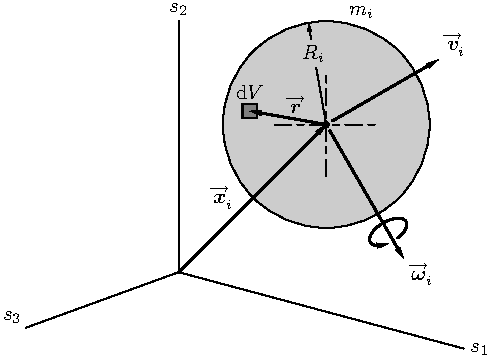
\includegraphics{figs/DEM-Def-Ball}
   \caption{Ball Element Parameters}
   \label{fig:BallDef}
\end{figure}


\subsection{Ball mass and inertia parameters}

Consider a volume element $\mathrm{d}V$ with respect to a static base $S$ of
an arbitrary solid body with  density $\rho$. The mass of the body is
obtained by integrating over the volume of the body,
\begin{equation}
    m = \int\limits_{\mathrm{body}} \rho\, \mathrm{d}V
    \label{eq:BMass-dif}
\end{equation}

In figure~\ref{fig:BallDef}, a ball with radius $R_{i}$ and uniform density
$\rho_i$ is depicted. The mass of the ball is after integration of
equation~\eqref{eq:BMass-dif}
\begin{equation}
    m_i = \tfrac{4}{3} \pi \rho_i\, R_i^3 .
    \label{eq:BMass}
\end{equation}


%----------------------------------------------------------------------------
\endinput
